\documentclass[12pt]{article}

\usepackage[english]{babel}
\usepackage[a4paper,top=2cm,bottom=2cm,left=3cm,right=3cm,marginparwidth=1.75cm]{geometry}

% Useful packages
\usepackage{amsmath}
\usepackage{graphicx}
\usepackage[colorlinks=true, allcolors=blue]{hyperref}
\usepackage{indentfirst}
%\usepackage{float}

\begin{document}

\title{CAUT: A Cellular Automata Simulation Framework for Parallel Programming Practice}
\author{Zacree Carroll, Troy Clendenen, Raul Patel}
\maketitle

\section{Abstract}
Our project aimed to find new ways to parallelize cellular automata. We began with what we considered to be a naive approach which essentially iterated across an entire grid of cells doing processing state updates even when some of those state updates had no chance of changing the state of that cell i.e. the cell had no live neighbors in its vicinity thus could not come to life. 
\par
The second approach we deemed the "Live Cell Relative Approach". This approach involved only looking at cells who were capable of coming to life on a given iteration thus saving time on the overhead of iterating the entire grid performing some unnecessary updates. Results initially seemed promising but we came to see that they were somewhat inconsistent. Because of this inconsistency we cannot definitively say that our Live Cell Relative algorithm in its current state can outperform the naive version.

\section{Introduction to Cellular Automata}
Cellular Automata (C.A.) are a very popular field of study and important framework when it comes to the realm of computational simulations. Its use spans the spectrum from simulating bio-remediation of contaminated soils to fluid flow simulations. CAMEL for example is a framework which abstracts away some of the hardware specifics of performing such computational simulations and allows the user to focus more time and energy on fine tuning their C.A. implementation. \cite{Cann95} A cellular automaton can be thought of as a collection of cells from which complex behaviors can arise from a relatively simple set of rules. As can be gathered from this view of C.A. it clearly is a very useful method for framing certain phenomena whose characteristics match the specification.

\section{Methodology}
Our goal with this project was to obviously get practice with parallel programming. So, we figured since many of our CA simulations we wanted to implement had already been done before, we did not want to look up how others implemented it until after we finished. So, we came up with 2 main approaches to how we could parallelize the simulations we wanted to.

\subsection{The Redundant Approach}
The simplest approach we could think of involved iterating across the entire m x n grid and perform some action on each cell in the grid. This action involves observing cells around the current cell in order to determine what the state of the current cell would be for the next iteration. Since we store the 'current' state and the 'next' state separately in memory, this allowed us to make changes to each cell on the grid completely independently, which turned the problem of parallelizing each generation of cells an embarassingly parallel problem.

On the downside (as you can assume based on the name of this approach), this meant that we were looking up the entire m x n grid, regardless of cell state. Usually in CA simulations, there are only a sparse set of cells that people care to observe. For example, if the user instantiated a grid of size 10,000 by 10,000, but there were only $<$10 active cells at any given time, that means that this algorithm is performing redundant work on the cells that aren't remotely close to these active cells, about 99.99\% of the work done is redundant. Cells in most CA simulations only affect the cells around them, and so we had to think of another approach that would potentially speed up our simulations significantly.

\subsection{The 'Live-Cell Relative' Approach}
There are a few main differences between the Live-Cell Relative (LCR) approach and the redundant approach. First, we initialized the grid with an array of pointers to all of the live cells that were instantiated by the user in the input file and assigned OpenMP threads to each of the cells in that array. This is not required in the previous approach. Another key difference is that the threads did not change the cell it was assigned to directly. Because we can obviously assume that the cells in the array are live, we update the next state of every cell around the live cell instead of the live cell itself. This works for most simulations because interesting interactions only ever happen around cells that are 'live'.

Because each OpenMP thread updates cells that are around live cells instead of the cell itself, this opens up a few possible race conditions. If 2 live cells are next to each other, and both OpenMP threads that are updating the cells around those both end up updating the same cell, we want to make sure that the value for that cell gets updated appropriatelly. This is easily solved with locks, and it's what we did in our implementation. However, the performance of this algorithm can vary a lot more, depending on if the grid is sparse in the number of live cells, or if the grid is dense in the number of live cells. If the grid has a higher live cell to dead cell ratio, the runtime of the program would actually be worse, because the race conditions introduced would mean that the cells are not being updated efficiently, and the benefit of only looking around live cells isn't as important, because most of the grid is live.

\section{Results}

\subsection{Game of Life}
First, let's show the results of the redundant algorithm on talapas. For this, we instantiated a grid of 4,000 x 4,000 where we randomly generated live cells at about a 1/10 chance.

\begin{figure}[ht]
\centering
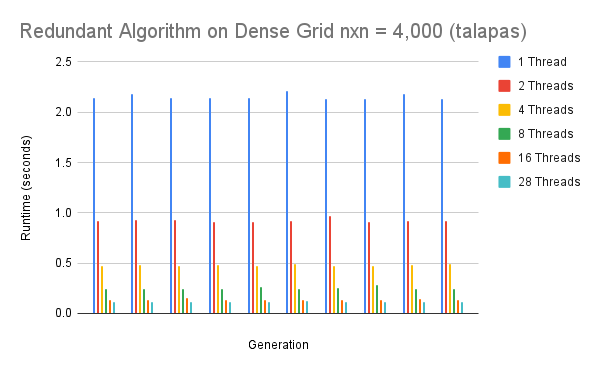
\includegraphics[width=\linewidth]{redundant_4000.PNG}
\caption{\label{fig:chart_1}Redundant algorithm results.}
\end{figure}

For the LCR algorithm, there is a much different trend in how performance differs based on the number of thread counts. Unfortunately, we were not able to test accurately on Talapas to compare the 2 algorithms. At some point in implementing the LCR algorithm, the runtime behavior for the redundant algorithm changed somehow, and we couldn't get consistent results. On our local machines, however, there were more readable results that still have merit, since they highlight the difference between the 2 algorithms. Listed below are both charts run on a Macbook Pro 2013 running Ubuntu natively, with an intel i5 chip.

\begin{figure}[ht]
\centering
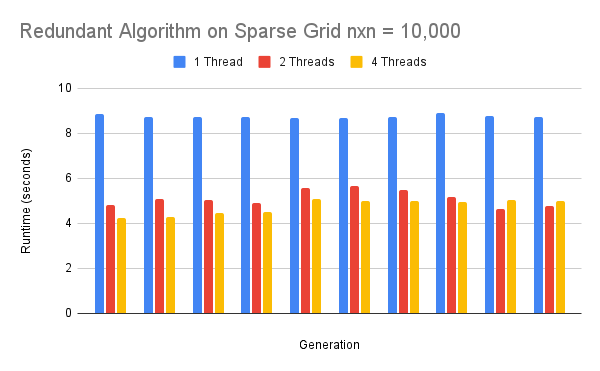
\includegraphics[width=\linewidth]{redundant_10000.PNG}
\caption{\label{fig:chart_2}Redundant algorithm results.}
\end{figure}

The above chart is the same algorithm as before, but on a grid of 10,000 x 10,000 cells. Note that we do not get a near-perfect speed improvement as we double the cores. 

\begin{figure}[!ht]
\centering
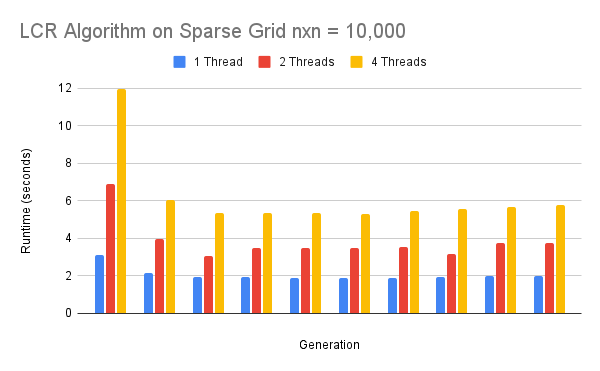
\includegraphics[width=\linewidth]{lcr_10000.PNG}
\caption{\label{fig:chart_3}Live-Cell Relative algorithm results.}
\end{figure}

Now there are quite a few things to unpack with the LCR results. Let's discuss some things before we talk about how increasing thread count actually made the run time of each generation even worse. First, the time it takes to go through each generation and update the cell's next state improves over the course of the program itself. This is due to 2 main reasons. First, given the fact that live cells have stricter rules regarding their 'liveness' means that most of the time, there are less live cells over the course of a simulation. The exceptions would be for large pulsars, many gliders, etc.

The next reason has to do with data that exists in cache. Because the LCR algorithm deals with cells that are nearby live cells, on the first iteration of the simulation, the vector for the live cells are in cache, but the location of these cells in the grid are not necessarily there. Because the Game of Life is predictable in where cells will appear for the next generation, we get to utilize spacial locality where cell activity goes on. When the 2nd generation of live cells are produced, the locations of those nearby cells are still in cache because we used them for the previous generation. Thus, as the program continues running, predicting where important cells are become easier, since the behavior of those cells become more clear as time goes on.

\subsection{Wildfire Simulations}

\subsubsection{Implementation}
For our wildfire simulation we wanted to keep it as simple as possible while also producing something that behaved in a way similar to how a wildfire would spread in real life. With a few simple rules and extra attributes in the cells we were able to accomplish something we felt looked good.
\par
The attributes we added were cell health/burnable material (0, 50] and a percentage of dry brush (0, 1] each initialized to a random value for every cell. The grid is initialized in a specific way so as to produce interesting output because a fire simulation where the fire does not spread is just not interesting. If a cell is not currently alive and still has hp and also has two neighbors that are alive then its chance to come alive/ignite is based on its percentage of dry brush it contains. If a cell is alive/on fire then it will lose a certain amount of its health every turn as would happen during a real fire. Both of these values were tinkered with a fair amount in an attempt to fine tune the fire spread to make it appear to be more realistic in the way that it moved through the cells. 
\par
Our sample runs for the fire simulation consisted of 20 runs at each thread count and each run calculated the simulation for roughly 50 iterations. We tried various grid sizes from 1,000 x 1,000 to 10,000 x 10,000 and eventually settled on a 5,000 x 5,000 size grid. The reason behind this is that we wanted a large enough grid that the amount of work to do was not trivial but also small enough that we did not spending days running our simulation to gather and compile our results. 
\subsubsection{Wildfire Results}
Unfortunately we ran into some very troubling issues when attempting to run our simulations on talapas. There were certain attempts that would never finish and others that would finish in a suspiciously short amount of time. However running locally we were not able to reproduce these problems on either of the two machines that we ran our simulations on. Below you will see a graph depicting run times via a Ryzen 5 2600x 6 core machine.
\begin{figure}[!ht]
    \centering
    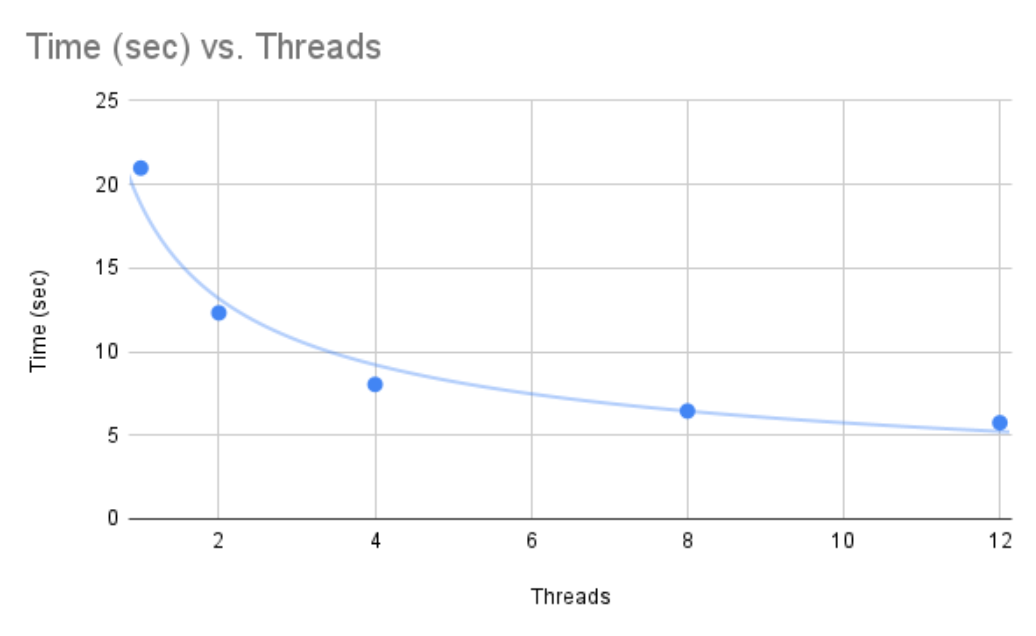
\includegraphics[width=\linewidth]{FireSimResGraph.PNG}
    \caption{Fire Simulation Performance Results}
    \label{fig:fireR}
\end{figure}
\par
As can be seen from the data we were able to achieve speed up with increasing the thread count for this algorithm which came as little surprise to us. We had planned to apply the Live Cell Relative approach to this algorithm given that it is not rule set specific however as mentioned previously we encountered some troubling issues there as well. However we speculate that the Live Cell Relative algorithm may not actually produce much speed up for the wildfire simulation because of how the cells tend to behave. Typically on what we would consider to be a useful/interesting trial of the simulation (i.e. the fire doesn't immediately burn out) large clusters of cells are alive simultaneously. This means that even if we only considered certain cells who have the potential to ignite at some point the Live Cell Relative algorithm would degenerate back into the naive approach where we are simply iterating through the entire grid.
\\

\subsection{Flocking Algorithms}

\section{Conclusion}

\bibliographystyle{alpha}
\bibliography{bibCol}

\end{document}
